% Chapter 4

\chapter{RICH Detector}
\label{ch:RICH} % For referencing the chapter elsewhere, use \autoref{ch:name}

%----------------------------------------------------------------------------------------

The particle identification is an important step in the hadron multiplicity extraction. In the COMPASS spectrometer it is performed by a large Ring Imaging Cherenkov detector (RICH) capable of separating pions, kaons and protons in a wide momentum range ( $\sim$$2$ GeV/$c$ to $\sim$$55$ GeV/$c$) and an angular aperture of $0.01$-$0.4$ radians.

In this chapter the RICH detection principle is presented as well as the description of its main components: the gas and mirror system, the photon detectors, the readout electronics and the data reconstruction.

\section{Cherenkov effect}

When a charged particle is moving through a transparent medium with a speed v greater than the speed of light (v$_{light} = c/n$, $n$ being the medium refractive index), a radiation known as \textit{Cherenkov radiation} is produced by the medium.

\begin{figure}[!h]
  \centering
	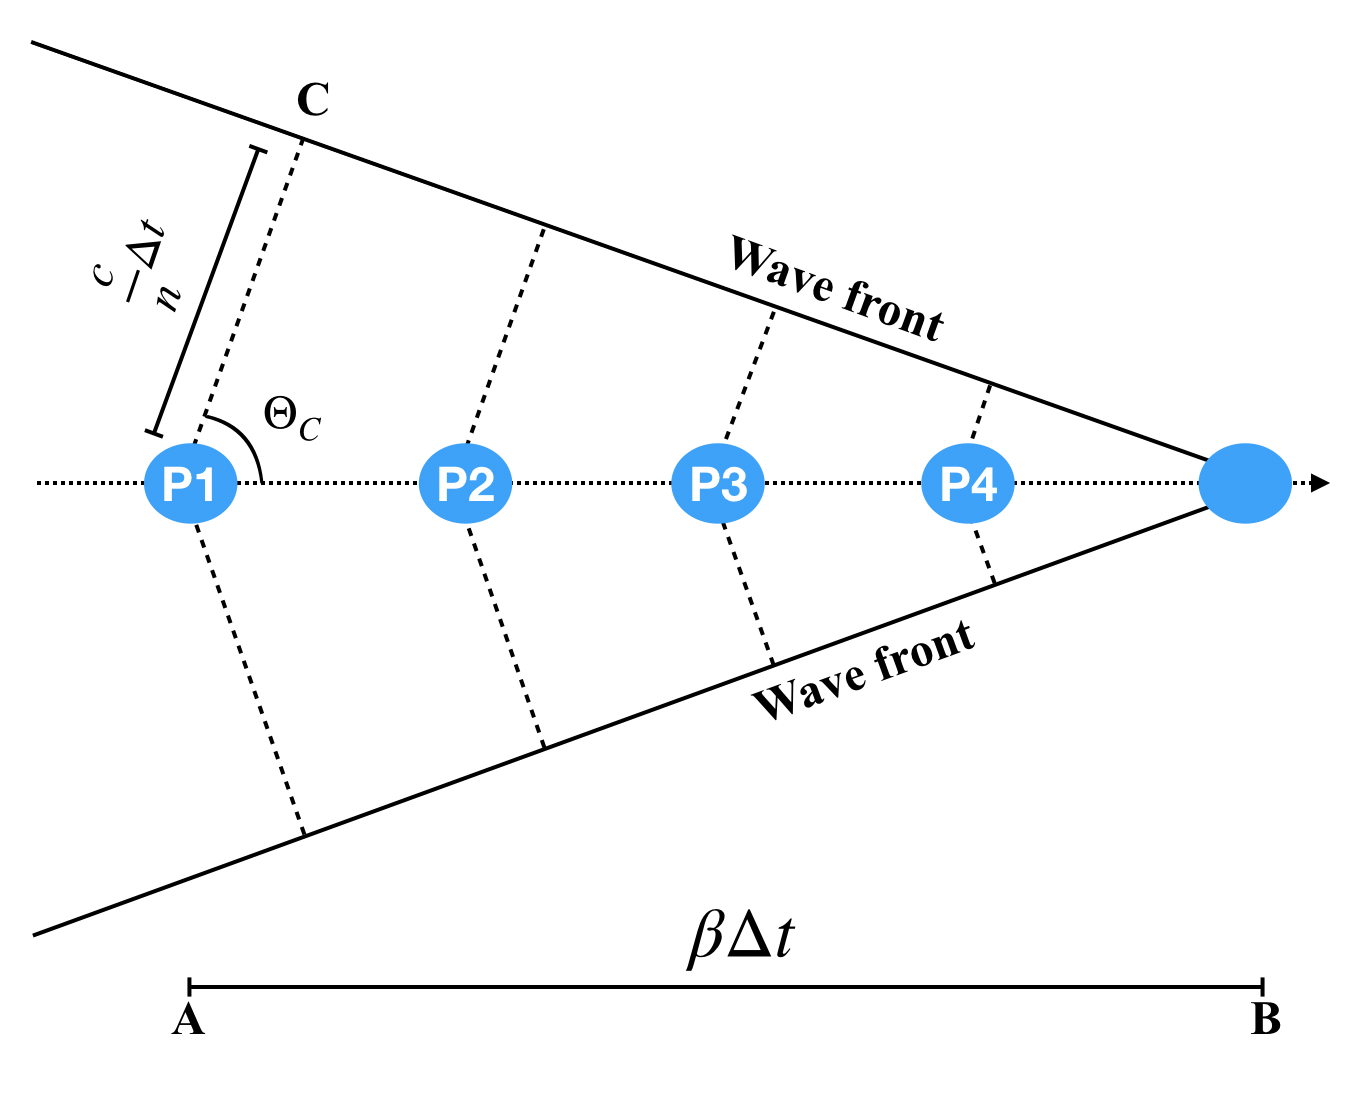
\includegraphics[scale=0.5]{./gfx/CherenkovGeom.png}
	\caption{Cherenkov radiation geometry.}
	\label{pic:CherenkovGeom}
\end{figure}

The Cherenkov radiation produced by a particle with a mass $M_h$ and momentum $p_h$ is emitted in a narrow cone around a particular angle $\Theta_C$ with respect to the particle track (Fig.~\ref{pic:CherenkovGeom}). The wavelength of these radiations goes from visible to UV.

The coherence between waves (emitted between A and B) is achieved, when the particle traverses $\overline{AB}$ at the same time as the radiation travels from A to C. The opening angle $\Theta_C$ is defined geometrically in Eq.~\ref{eq:thetaC} with $\beta$ being the particle velocity over the speed of light.
%
\begin{equation}
  cos\Theta_C = \frac{c/n \Delta t}{\beta c \Delta t} = \frac{1}{n\beta}
  \label{eq:thetaC}
\end{equation}
%
Some limit cases can be devised:
\begin{enumerate}
  \item Threshold limit: if $\beta \leq 1/n$ no Cherenkov radiation will be emitted.
  \item Maximum emission angle: $cos \Theta_C = \frac{1}{n}$ is reached for ultra-relativistic particles ($\beta = 1$).
\end{enumerate}

In order to perform particle identification with a RICH detector, two variables have to be measured: $\Theta_C$ and $p_h$. The angle can be measured detecting the emitted photons. Different techniques can be used to collect and transport the produced photons to the location of the light detectors. The resulting image in the detector plane is a ring, only for specific techniques, if one does a proper optical image. In such a case the ring has a radius proportional to $\Theta_C$. $p_h$ is measured independently by the spectrometer. The particle mass can thus be calculated by:
%
\begin{equation}
  M_h = p_h \sqrt{n^2 cos^2 \Theta_C -1}
\end{equation}

%------------------------------------------------

\section{The COMPASS RICH detector}

The COMPASS RICH detector is designed to distinguish between pions, kaons and protons at high intensities. The momentum range covers the pion Cherenkov threshold ($\sim$ $2.67$ GeV/c) to $\sim$ $55$ GeV/c.

The RICH is a large size detector ($\sim$ $3$ x $5$ x $6$ m$^3$, see Fig.~\ref{pic:RICHview}) filled with a gaseous radiator. Two spherical mirror systems reflect the photons into an array of photon detectors sensitive to a large wavelength range, from visible to far UV, placed outside the spectrometer acceptance, one above and one below the beam line. The goal is to count as many photons as possible with a good spacial resolution. The whole structure of the detector vessel is built mainly in thin aluminium in order to minimize the material budget.

Until $2004$, MultiWire Proportional Chambers (MWPC) equipped with solid-state CsI photo-cathodes were used to detect Cherenkov photons. The gains of the MWPC operation was limited. The first stage of the electronic readout was characterized by a long integration time, which was a limiting factor in the COMPASS environment as there is a high-rate uncorrelated background due to the large muon halo beam. Moreover, the long base-line restoration time generated a non-negligible dead time. To overcome these limitations, the central region that covers $25$\% of the photo-detection surface was replaced with MultiAnode PhotoMultiplier Tubes (MAPMT). They are intrisically fast and have better time resolutions.

\begin{figure}[!h]
  \centering
	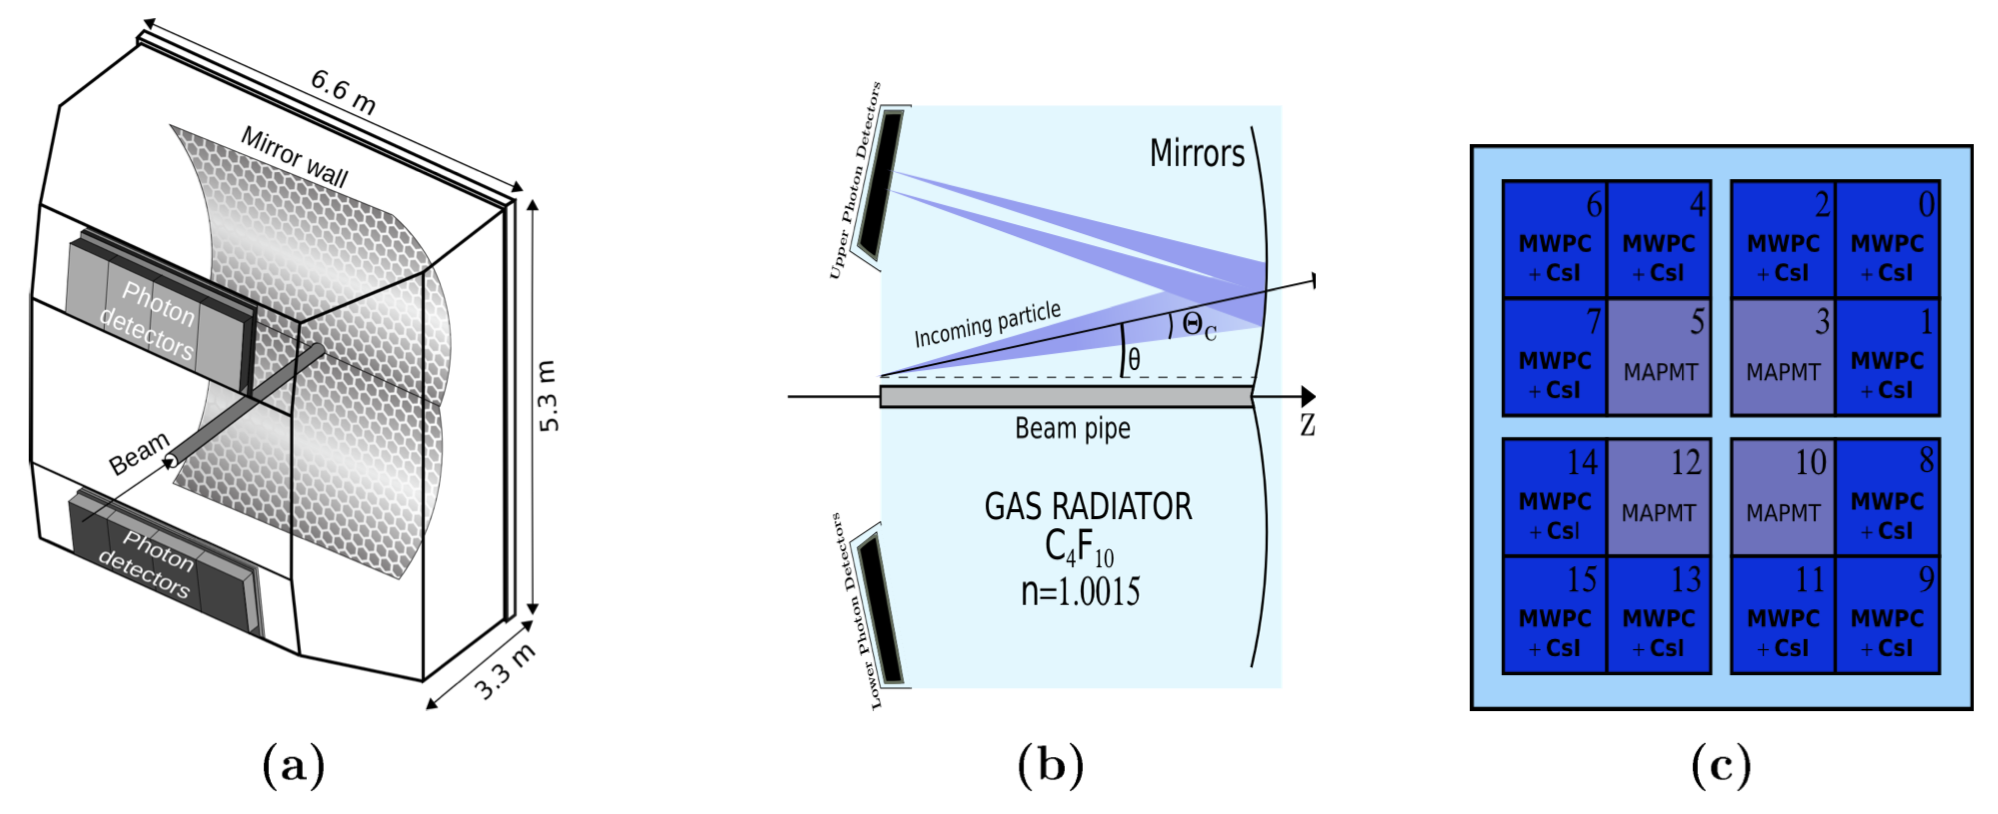
\includegraphics[scale=0.4]{./gfx/RICHview.png}
	\caption{(a) Artistic view of the COMPASS RICH detector. (b) Basic functioning of the RICH detector. (c) Photon detector disposition (not to scale).}
	\label{pic:RICHview}
\end{figure}

\subsection{Gas System}

One of the principal elements of a RICH detector is the radiator. At COMPASS it is perfluorobutane (C$_4$F$_{10}$). It has a refractive index of n $\approx$ $1.0015$ and a low chromaticity\footnote{Dependence of the refractive index of a dielectric medium on the photon wavelength \cite{Dispersion}} ($dn/dE_{\gamma}$ of about $5 \cdot 10^{-5}$~eV$^{-1}$). These characteristics allow the particle identification (PID) to be performed in the aforementioned wide momentum range.

The propagation of the Cherenkov photons in the vessel can be affected by the presence of water vapor and oxygen (high UV light absorption cross section). In order to remove these impurities, the gas is constantly circulating and filtered at a constant pressure (1 mbar higher than the atmospheric pressure) in a dedicated gas system \cite{RICHGas}. The overpressure of the vessel is needed to prevent air contamination and to avoid mechanical stress to the detector, given its large size. Other circulation system (known as \textit{fast circulation} system) allows a reshuffling of the gas inside the vessel: as perfluorobutane has a density of $11.21$ kg/m$^3$ it avoids stratification that may cause a gradient in the value of the refractive index from top to bottom.

In order to absorb the photon emitted by the muon beam, a $10$ cm diameter pipe filled with helium is positioned inside the vessel along the beam.

\subsection{Mirror System}

The RICH optical system covers an area of $\sim$ $21$ m$^2$ and consists of two spherical surfaces, each one containing $58$ spherical mirrors of different shapes ($34$ hexagons and $24$ pentagons). The mirror pattern is shown in Fig.~\ref{pic:RICHmirrors}. All the mirrors have a reflectance above $80$\% in the UV region.

The mirror system has a radius of curvature of $6.6$ m. The photon image is focused outside the spectrometer acceptance where the photon detectors are located. As the radii of the curvature have a scatter of $1$\% (R = $6600\pm66$ mm), the reflected image is slightly blurred. This effect is more pronounced for particles at large angles \cite{RICHMirror}: this aberration contributes to the dispersion of the photon angle with respect to the angle of emission, which affects the detection resolution \cite{RICHPID}.

\begin{figure}[!h]
  \centering
	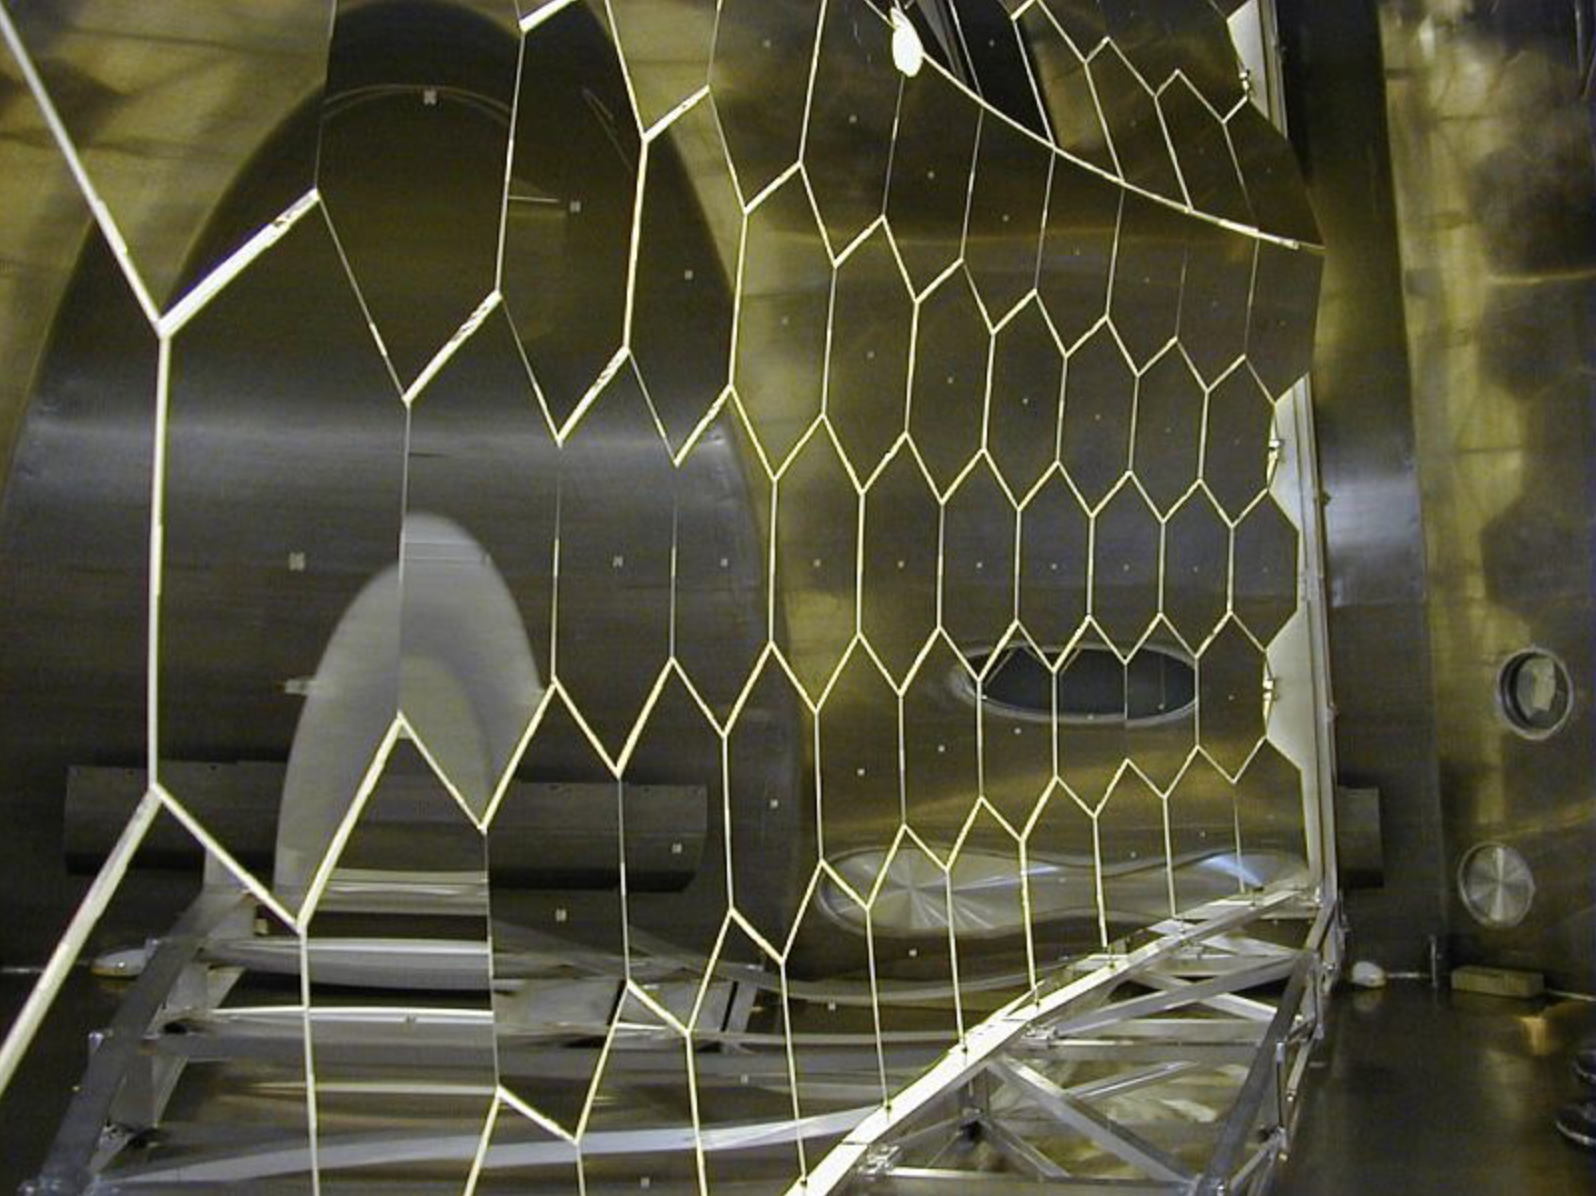
\includegraphics[scale=0.4]{./gfx/RICHmirrors.png}
	\caption{COMPASS RICH detector optical system.}
	\label{pic:RICHmirrors}
\end{figure}

\subsection{Photon Detectors}

The photon detector array consists of two symmetric parts with respect to the beam line, each one is composed of $8$ modules located at the mirror focal plane. The modules in the external regions are MultiWire Proportional Chambers (MWPC) equipped with solid state CsI photo-cathodes \cite{RICHLimits}. The central area is composed by MultiAnode Photomultiplier Tubes (MAPMT) \cite{RICHUpgrade} coupled to individual telescopes of fused silica lenses. The use of two different detector types employing different different photon converters results in the detection of photons in two wavelength regions: < $200$ nm for MWPCs and $\sim$ $200$ - $650$ nm for MAPMT. The low momentum particles are mainly detected by the outer part (MWPC), while the high momentum ones are detected by the central part (MAPMT). Only the central part is used in the following analysis.

The spherical mirrors will focus all the photons emitted parallel in the same point. Thus the Cherenkov light cone of our particle will result in a ring at the detector plane. The distribution of photons in the detectors for a physics event is shown in Fig.~\ref{pic:RICHEvent}.

\begin{figure}[!h]
  \centering
	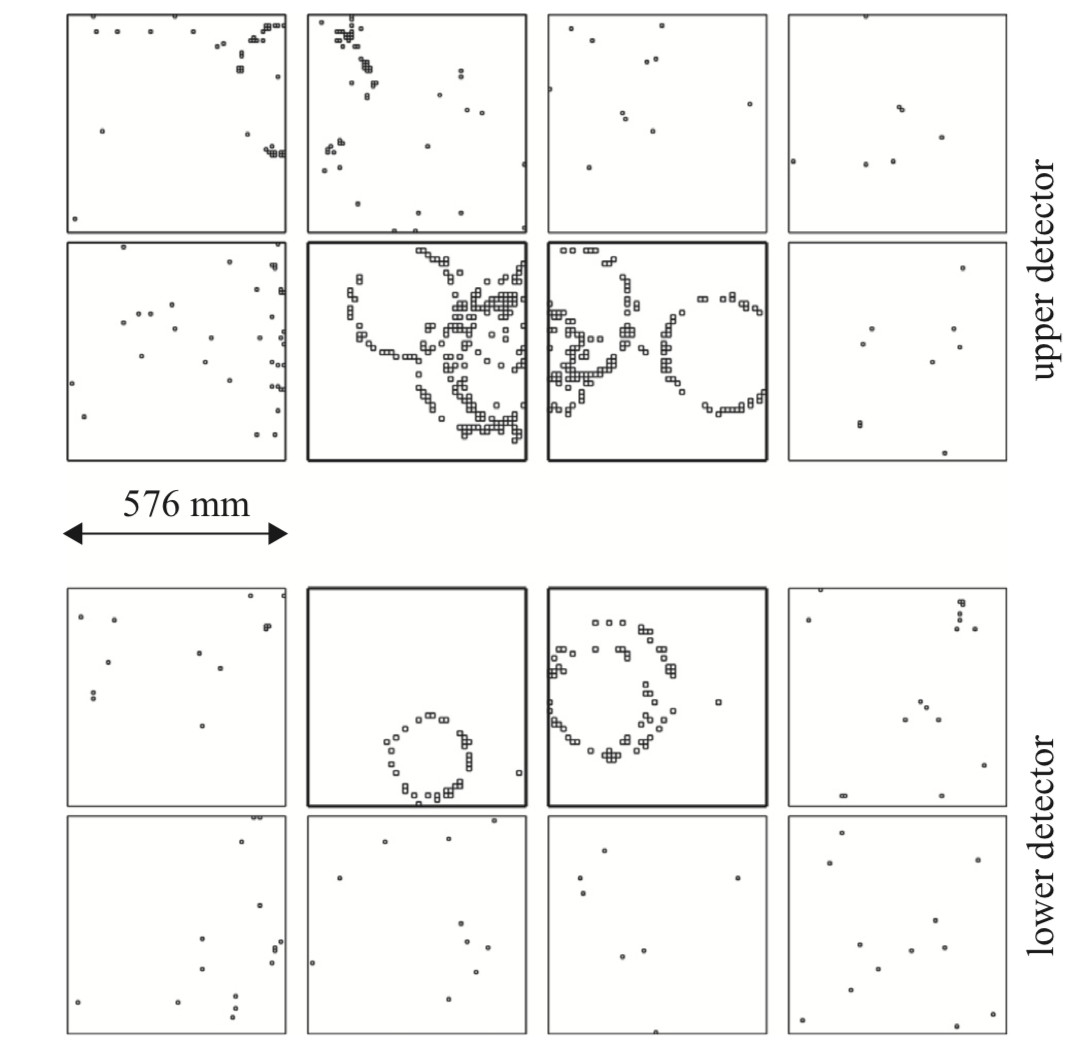
\includegraphics[scale=0.5]{./gfx/RICHEvent.png}
	\caption{An event from the online event display of COMPASS RICHONE. The $16$ squares represent the detectors areas ; the four central ones are equipped with MAPMTs. the small squares represent the hits with signal amplitudes larger than a threshold, individually set for each channel. Figure taken from \cite{NIM2015}}
	\label{pic:RICHEvent}
\end{figure}

\subsection{RICH Infos Reconstruction}

RICHONE is a package contained in the CORAL software, which is in charge of RICH information reconstruction. The reconstruction is divided in several parts, the first being decoding the data and clustering. Then the reconstruction of the Cherenkov angle for each individual photon is done. It is possible to perform a ring reconstruction which is used for studies on the apparatus. The particle identification (PID) is based on a maximum likelihood calculation. The PID will be explained more thouroughly afterwards.

\subsubsection*{Decoding and clustering}

There are two different types of photon detectors and they have different decoding systems and clustering algorithms. For the MWPCs, if more than one channel fires, a clustering is done. When the pad with the highest pulse height is found, all the adjacent pads with a smaller signal are included in the cluster \cite{RICHPID}. The mean position of each active pad is evaluated in the cluster, weighting the signal with their maximum pulse height, to determine the center of gravity of the cluster. For the MAPMT, decoding the signal is enough to read the time information coming from the PMT that was hit. As the probability of having correlated hits in adjacent area is negligible, the MAPMT data does not need clustering \cite{RICHElec}.

The cluster or hit position is used to determine the trajectory of the photon. In addition, the time information coming from the MAPMT is used to reject out-of-time photons while the amplitude information from the MWPC serves to reduce the background both from out-of-time photons and from electronic noise \cite{RICHPID}.

\subsubsection*{Cherenkov angle and ring reconstruction}

The ring reconstruction begins with the selection of a particle tracks. Then one looks for the photons around this track. The trajectory of each Cherenkov photon is calculated with respect to the plane containing the particle track and its virtual reflection in the mirror in order to reconstruct $\Theta_C$ \cite{RICHTheory}. All the photons emitted by one particle are expected to have the same angle $\Theta_C$ and to be uniformly distributed in $\phi$. The photons emitted by other particles or from background have on the contrary a flat $\Theta_C$ distribution. The emitted photon with the same ($\Theta_C$,$\phi$) pair are reflected on the same location at the focal surface (neglecting any spherical aberration), resulting in a ring image of the photon detector. Since the emission point of the photon along the particle trajectory is not known, the middle point between the detector and the mirror is taken. A good determination of the track trajectory parameters and the momentum of the particle are mandatory in order to extract $\Theta_C$ with good precision.

To characterize the RICH, determining its angular resolution for instance, the ring reconstruction of the emitted photons is needed. The ring reconstruction is based on the search of a peak in the $\Theta_C$ distribution. Small intervals of $\pm$3$\sigma$ ($\sigma$ being the single photon resolution, $\sigma_{MAPMT}$ = $2.0$ mrad and $\sigma_{MWPC}$ = $2.5$ mrad) on an overall range of $0$ to $70$ mrad are considered. The interval with the maximum number of entries is used to define the ring. This procedure associates a ring to each track and in order to reject tracks with only background photons a minimal amount of photons per ring is required (four photons for the MAPMT part) \cite{RICHPID}. The resolution of the Cherenkov angle measurement provided by each single photon as a function of the particle momentum is illustrated in Fig.~\ref{pic:RICHRez}.

\begin{figure}[!h]
  \centering
	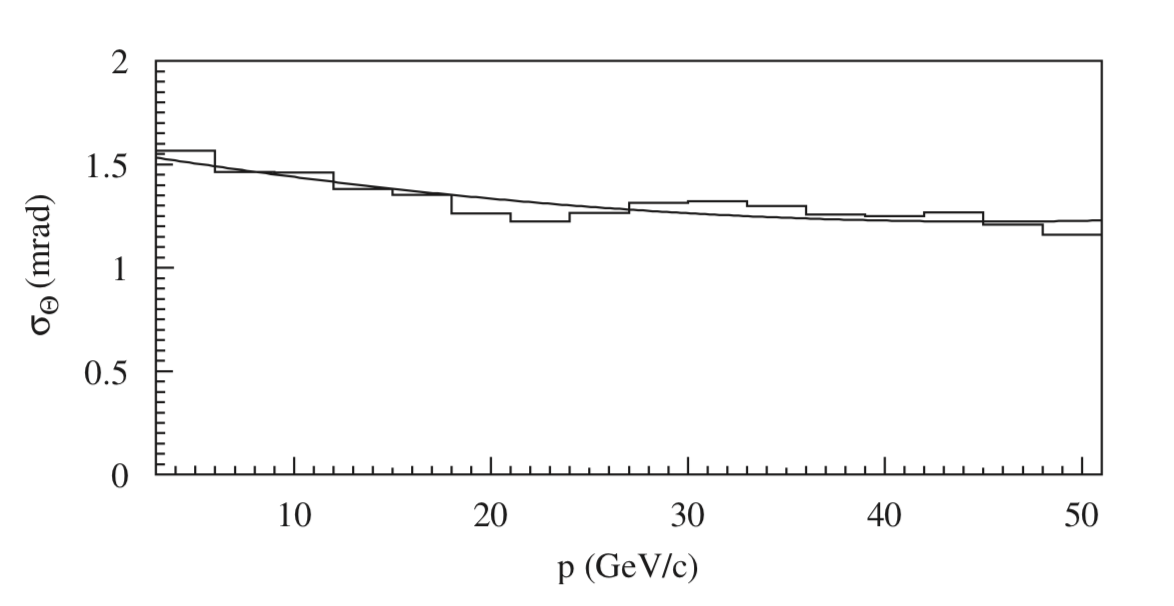
\includegraphics[scale=0.5]{./gfx/RICHRez.png}
	\caption{Resolution of the Cherenkov angle for the reconstructed ring images, provided by each single photon, versus the particle momentum for a sample of identified pions. Figure taken from \cite{NIM}.}
	\label{pic:RICHRez}
\end{figure}

The measured values of $\theta_C$ as a function of $p_h$ for the RICH detector are shown in Fig.~\ref{pic:RICH}. In the low momentum region, the RICH detector is only sensitive to electrons, muons and pions. The bands corresponding to kaons and protons start to be visible respectively at $p_h \approx$ $9.45$ GeV/c and $p_h \approx$ $17.95$ GeV/c. For high momentum values above $40$ GeV/c, saturation of the Cherenkov angle is observed or pions and kaons. The final particle identification is performed using likelihood methods and is described in the following chapter.

\begin{figure}[!h]
  \centering
	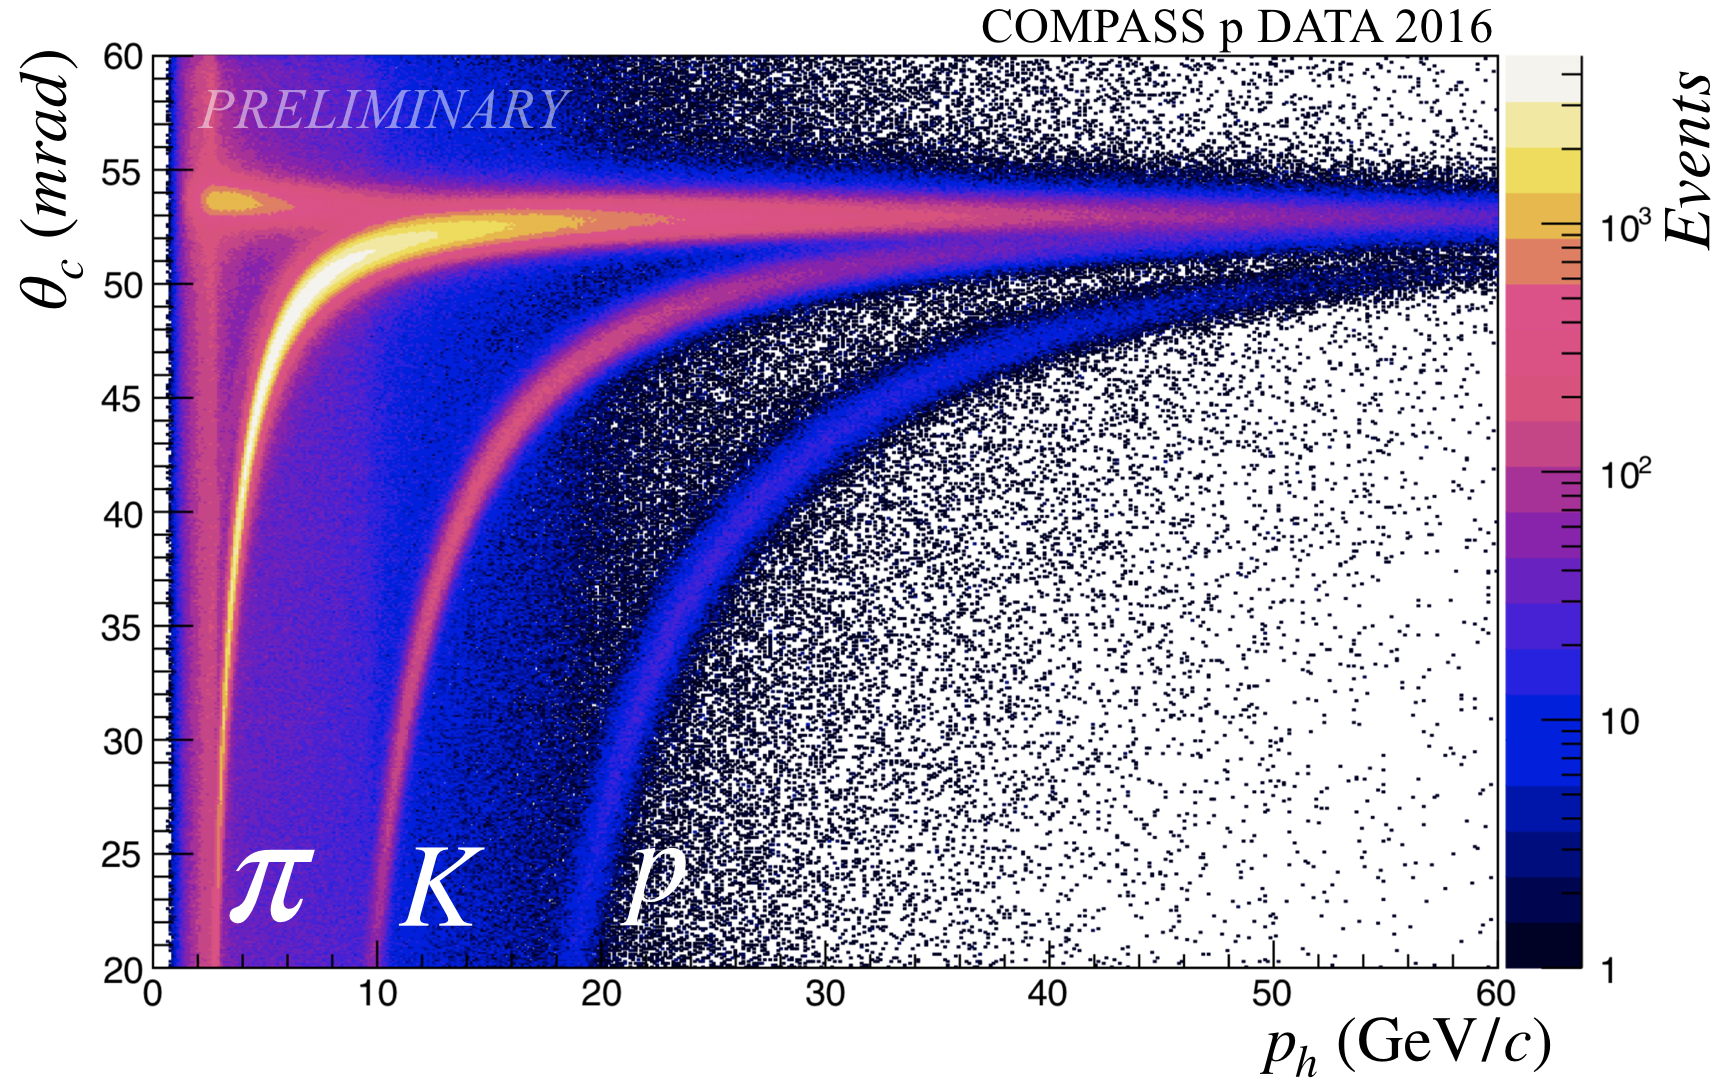
\includegraphics[scale=0.45]{./gfx/RICH.png}
	\caption{Measured Cherenkov angle $\Theta_C$ as a function of $p_h$. $\pi$ threshold is about $2.67$ GeV/$c$, $K$ threshold about $9.45$ GeV/$c$ and $p$ threshold about $17.95$ GeV/$c$, respectively.}
	\label{pic:RICH}
\end{figure}
